\label{sec:pup}

The \index{PUP} PUP framework is a generic way to describe the data in an object and to use that description for any task requiring serialization.
The \charmpp\ system can use this description to pack the object 
into a message, and unpack the message into a new object on another 
processor. 
The name thus is a contraction of the words Pack and UnPack (PUP). 

Like many \CC\ concepts, the PUP framework is easier to use than 
describe: 

\begin{alltt}
class foo : public mySuperclass \{
 private:
    double a;
    int x;
    char y;
    unsigned long z;
    float arr[3];
 public:
    ...other methods...

    //pack/unpack method: describe my fields to charm++
    void pup(PUP::er &p) \{
      mySuperclass::pup(p);
      p|a;
      p|x; p|y; p|z;
      PUParray(p,arr,3);
    \}
\};
\end{alltt}

This class's \uw{pup} method describes the fields of a \uw{foo} to \charmpp{}.
This allows \charmpp\ to: marshall parameters of type \uw{foo} across processors,
translate \uw{foo}s across processor architectures, read and write \uw{foo}s
to disk files, inspect and modify \uw{foo} objects in the debugger, and 
checkpoint and restart calculations involving \uw{foo}s.



\section{PUP contract}

\label{sec:pupcontract}
Your object's \uw{pup} method must save and restore all your object's
data.  As shown, you save and restore a class's contents by writing a
method called ``pup'' which passes all the parts of the class to an
object of type \index{PUP::er} \kw{PUP::er}, which does the saving or
restoring.  This manual will often use ``pup'' as a verb, meaning ``to
save/restore the value of'' or equivalently, ``to call the pup method
of''.

Pup methods for complicated objects normally call the pup methods
for their simpler parts.  Since all objects depend on their immediate
superclass, the first line of every pup method is a call to the 
superclass's pup method---the only time you shouldn't call your superclass's
pup method is when you don't have a superclass.  If your superclass has
no pup method, you must pup the values in the superclass yourself.


\subsection{PUP operator}
\label{sec:pupoperator}

The recommended way to pup any object \verb.a. is to use \verb.p|a;..
This syntax is an operator \verb.|. applied to the \kw{PUP::er} \verb.p.
and the user variable \verb.a..

The \verb.p|a;. syntax works wherever \verb.a. is:

\begin{itemize}
 \item A simple type, including char, short, int, long, float, or double.
    In this case, \verb.p|a;. copies the data in-place.
    This is equivalent to passing the type directly to the \kw{PUP::er}   
       using \verb.p(a)..
 \item Any object with a pup method.
    In this case, \verb.p|a;. calls the object's pup method.
    This is equivalent to the statement \kw{a.pup(p);}. 
 \item A pointer to a PUP::able object, as described in Section~\ref{sec:pup::able}.
    In this case, \verb.p|a;. allocates and copies the appropriate subclass.
 \item An object with a \kw{PUPbytes}(\uw{myClass}) declaration in the header.
    In this case, \verb.p|a;. copies the object as plain bytes, like memcpy.
 \item An object with a custom \verb.operator |. defined.
    In this case, \verb.p|a;. calls the custom \verb.operator |..
\end{itemize}

See \examplerefdir{PUP}

For container types, you must simply pup each element of the container.
For arrays, you can use the utility method \kw{PUParray}, which takes
the \kw{PUP::er}, the array base pointer, and the array length.
This utility method is defined for user-defined types T as:
  \begin{alltt}
    template<class T>
    inline void PUParray(PUP::er &p,T *array,int length) \{
       for (int i=0;i<length;i++) p|array[i];
    \}
  \end{alltt}


\subsection{PUP STL Container Objects}
\label{sec:pupstl}
If the variable is from the C++ Standard Template Library, you can include 
operator\verb.|.'s for STL vector, map, list, pair, and string, templated
on anything, by including the header ``pup\_stl.h''.

See \examplerefdir{PUP/STLPUP}

\subsection{PUP Dynamic Data}
As usual in \CC{}, pointers and allocatable objects usually require special handling. 
Typically this only requires a \kw{p.isUnpacking()} conditional block, 
where you perform the appropriate allocation.  See 
Section~\ref{sec:pupdynalloc} for more information and examples.  

If the object does not have a pup method, and you cannot add one or use 
PUPbytes, you can define an operator\verb.|. to pup the object.
For example, if \uw{myClass} contains two fields \uw{a} and \uw{b}, the 
operator\verb.|. might look like:

\begin{alltt}
  inline void operator|(PUP::er &p,myClass &c) \{
    p|c.a;
    p|c.b;
  \}
\end{alltt}

See \examplerefdir{PUP/HeapPUP}

\subsection{PUP as bytes}

\label{sec:pupbytes}

For classes and structs with many fields, it can be tedious and 
error-prone to list all the fields in the pup method.
You can avoid this listing in two ways, as long as the
object can be safely copied as raw bytes---this is normally 
the case for simple structs and classes without pointers.

\begin{itemize}
\item Use the \verb.PUPbytes(myClass). macro in your header file.
      This lets you use the \verb.p|*myPtr;. syntax 
      to pup the entire class as sizeof(myClass) raw bytes.

\item Use \verb.p((void *)myPtr,sizeof(myClass));. in the pup 
      method.  This is a direct call to pup a set of bytes. 
      
\item Use \verb.p((char *)myCharArray,arraySize);. in the pup 
      method.  This is a direct call to pup a set of bytes. 
	  Other primitive types may also be used.
      
\end{itemize}

Note that pupping as bytes is just like using `memcpy': 
it does nothing to the data other than copy it whole.
For example, if the class contains any pointers, you
must make sure to do any allocation needed, and
pup the referenced data yourself.

Pupping as bytes may prevent your pup method from ever being able to
work across different machine architectures.  This is currently
an uncommon scenario, but heterogenous architectures may become more
common, so pupping as bytes is discouraged.

\subsection{PUP overhead}

\label{sec:pupoverhead}

The \kw{PUP::er} overhead is very small---one virtual function call
for each item or array to be packed/unpacked.  The actual packing/unpacking is
normally a simple memory-to-memory binary copy. 

For arrays of builtin types like ``int" and ``double", or arrays of a type 
with the ``PUPbytes'' declaration, \kw{PUParray} uses an even faster block 
transfer, with one virtual function call per array.


\subsection{PUP structured dagger}

\label{sec:pupsdag}

Please note that if your object contains Structured Dagger code (see section~\ref{sec:sdag}) you must call the generated method \kw{\_\_sdag\_pup}, after any superclass pup methods, to correctly pup the Structured Dagger state:

\begin{alltt}
class bar : public barParent \{
 public:
    bar_SDAG_CODE 
    ...other methods...

    virtual void pup(PUP::er& p) \{
      barParent::pup(p);
      __sdag_pup(p);
      ...pup other data here...
    \}
\};
\end{alltt}



\subsection{PUP modes}

\label{sec:pupmodes}

\charmpp{} uses your pup method to both pack and unpack, 
by passing different types of \kw{PUP::er}s to it.  The method
\kw{p.isUnpacking()} returns true if your object is being unpacked---that 
is, your object's values are being restored.  Your pup method must
work properly in sizing, packing, and unpacking modes; and
to save and restore properly, the same fields must be passed 
to the \kw{PUP::er}, in the exact same order, in all modes.
This means most pup methods can ignore the pup mode.

Three modes are used, with three separate types of \kw{PUP::er}: 
sizing, which only computes the size of your data without modifying it;
packing, which reads/saves values out of your data; and unpacking,
which writes/restores values into your data.  You can determine
exactly which type of \kw{PUP::er} was passed to you using the
\kw{p.isSizing()}, \kw{p.isPacking()}, and \kw{p.isUnpacking()}
methods. However, sizing and packing should almost always be 
handled identically, so most programs should use \kw{p.isUnpacking()}
and \kw{!p.isUnpacking()}.  Any program that calls \kw{p.isPacking()} 
and does not also call \kw{p.isSizing()} is probably buggy, because
sizing and packing must see exactly the same data.


The \kw{p.isDeleting()} flag indicates the object will be deleted
after calling the pup method.  This is normally only needed for
pup methods called via the C or f90 interface, as provided by 
AMPI or the other frameworks.  Other \charmpp{} array elements, 
marshalled parameters, and other C++ interface objects 
have their destructor called when they are deleted, so the 
\kw{p.isDeleting()} call is not normally required---instead,
memory should be deallocated in the destructor as usual.

More specialized modes and PUP::ers are described in section~\ref{sec:PUP:CommonPUPers}. 


\section{PUP Usage Sequence}

\label{sec:lifecycle}

\begin{figure}[h]
\begin{center}
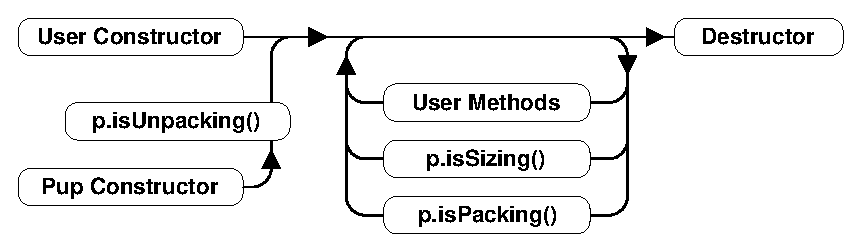
\includegraphics[width=6.0in]{fig/pup}
\end{center}
\caption{Method sequence of an object with a pup method.}
\label{fig:pup}
\end{figure}

Typical method invocation sequence of an object with a pup method is shown in 
Figure~\ref{fig:pup}.  As usual in \CC{}, objects are 
constructed, do some processing, and are then destroyed.

Objects can be created in one of two ways: they can
be created using a normal constructor as usual; or they
can be created using their pup constructor.  The pup constructor
for \charmpp{} array elements and \kw{PUP::able} objects
is a ``migration constructor'' that takes a single ``CkMigrateMessage *";
for other objects, such as parameter marshalled objects,
the pup constructor has no parameters.  The pup constructor
is always followed by a call to the object's pup method in
\verb.isUnpacking. mode.

Once objects are created, they respond to regular user methods
and remote entry methods as usual.  At any time, the object 
pup method can be called in \verb.isSizing. or \verb.isPacking.
mode.  User methods and sizing or packing pup methods can be called
repeatedly over the object lifetime.

Finally, objects are destroyed by calling their destructor
as usual.


\section{Migratable Array Elements using PUP}

\label{arraymigratable}
Array objects can \index{migrate}migrate from one PE to another.  For
example, the load balancer (see section~\ref{lbFramework}) might
migrate array elements to better balance the load between processors.
For an array element to be migratable, it must implement a \uw{pup}
method.  The standard PUP contract (see section \ref{sec:pupcontract})
and constraints wrt to serializing data, and use of Structured Dagger
apply. 


A simple example for an array follows:

\begin{alltt}
//In the .h file:
class A2 : public CBase\_A2 \{
private: //My data members:
    int nt;
    unsigned char chr;
    float flt[7];
    int numDbl;
    double *dbl;
public:	
    //...other declarations

    virtual void pup(PUP::er \&p);
\};

//In the .C file:
void A2::pup(PUP::er \&p)
\{
    CBase\_A2::pup(p); //<- MUST call superclass's pup method
    p|nt;
    p|chr;
    p(flt,7);
    p|numDbl;
    if (p.isUnpacking()) dbl=new double[numDbl];
    p(dbl,numDbl);
\}
\end{alltt}

The default assumption, as used in the example above, for the object
state at PUP time is that a chare, and its member objects, could be
migrated at any time while it is inactive, i.e. not executing an entry
method.  Actual migration time can be controlled (see
section~\ref{lbFramework}) to be less frequent.  If migration timing
is fully user controlled, e.g., at the end of a synchronized load
balancing step, then PUP implementation can be simplified to only
transport ``live'' ephemeral data matching the object state which
coincides with migration.  More intricate state based PUPing, for
objects whose memory footprint varies substantially with computation
phase, can be handled by explicitly maintaining the object's phase in
a member variable and implementing phase conditional logic in the PUP
method (see section~\ref{sec:pupdynalloc}).

\section{Marshalling User Defined Data Types via PUP}

Parameter marshalling requires serialization and is therefore
implemented using the PUP framework.  User defined data types passed
as parameters must abide by the standard PUP contract (see section
\ref{sec:pupcontract}).

For efficiency, arrays are always copied as blocks of bytes and passed
via pointers.  This means classes that need their pup routines to be
called, such as those with dynamically allocated data or virtual
methods cannot be passed as arrays--use CkVec or STL vectors to pass
lists of complicated user-defined classes.  For historical reasons,
pointer-accessible structures cannot appear alone in the parameter
list (because they are confused with messages).

The order of marshalling operations on the send side is:
\begin{itemize}
\item Call ``p\verb.|.a'' on each marshalled parameter with a sizing PUP::er.
\item Compute the lengths of each array.
\item Call ``p\verb.|.a'' on each marshalled parameter with a packing PUP::er.
\item \kw{memcpy} each arrays' data.
\end{itemize}

The order of marshalling operations on the receive side is:
\begin{itemize}
\item Create an instance of each marshalled parameter using its default constructor.
\item Call ``p\verb.|.a'' on each marshalled parameter using an unpacking PUP::er.
\item Compute pointers into the message for each array.
\end{itemize}

Finally, very large structures are most efficiently passed via messages,
because messages are an efficient, low-level construct that minimizes copying
and overhead; but very complicated structures are often most easily passed via 
marshalling, because marshalling uses the high-level pup framework.

See \examplerefdir{PUP/HeapPUP}

